\documentclass{beamer}


\usepackage[no-math]{fontspec}
\usepackage{xunicode}
\usepackage{xltxtra}
\usepackage{tikz}
\usepackage{graphicx}
\usepackage{booktabs}
\usepackage{fontawesome}
\usepackage[normalem]{ulem}
\usepackage[mode=text]{siunitx}
\usepackage{hyperref}


% Beamer setup
\mode<presentation>
{
	\usetheme{OtagoPlain}
	\setbeamertemplate{navigation symbols}{}
}


% TikZ setup
\usetikzlibrary{positioning}
\usetikzlibrary{calc}
\usetikzlibrary{arrows.meta}
\usetikzlibrary{shapes.geometric}


% fontspec setup
\defaultfontfeatures{Mapping=tex-text}
\setmainfont{Minion Pro}
\setsansfont[Scale=MatchUppercase,BoldFont={Open Sans}]{Open Sans Light}
\setmonofont[Scale=MatchLowercase]{Letter Gothic 12 Pitch}


% graphicx setup
\graphicspath{{images/}}


% misc
\newcommand{\todo}[1]{\alert{\textbf{!!TODO!! [#1] !!}}}


% Draw a grid to aid TikZ picture drawing/debugging.
\newcommand{\DrawGridTikZ}[2]{%
	\begin{scope}[color=lightgray]
		\draw[thin,step=1mm]  (0.0,0.0)   grid (#1,#2);%
		\draw[thick,step=1cm] (-0.1,-0.1) grid (#1+0.1,#2+0.1);%
		\pgftext[top,at={\pgfxy(0.0,-0.2)}]{\tiny 0}%
		\pgftext[right,at={\pgfxy(-0.2,0.0)}]{\tiny 0}%
		\foreach \x in {1,...,#1} {\pgftext[top,at={\pgfxy(\x,-0.2)}]{\tiny\x}}%
		\foreach \y in {1,...,#2} {\pgftext[right,at={\pgfxy(-0.2,\y)}]{\tiny\y}}%
	\end{scope}
}


% Sometimes we want to put a comment in tiny text on the next line, but the default line skip
% will insert too much vertical space. Put a \tinyskip at the end of the line instead.
\def\tinyskip{\\[-0.33\baselineskip]}


% Bold-face text using the structure colour.
\newcommand<>{\structurebf}[1]{\structure#2{\textbf{#1}}}


% preamble
\title{Adventures in data wrangling}
\author{Nigel Stanger}
\date{July 20, 2018}


\begin{document}


%%%%%%%%%%%%%%%%%%%%%%%%%%%%%%%%%%%%%%%%%%%%%%%%%%%%%%%%%%%%%%%%%%%%%%%%%%%%%%%%


\setbeamertemplate{background canvas}{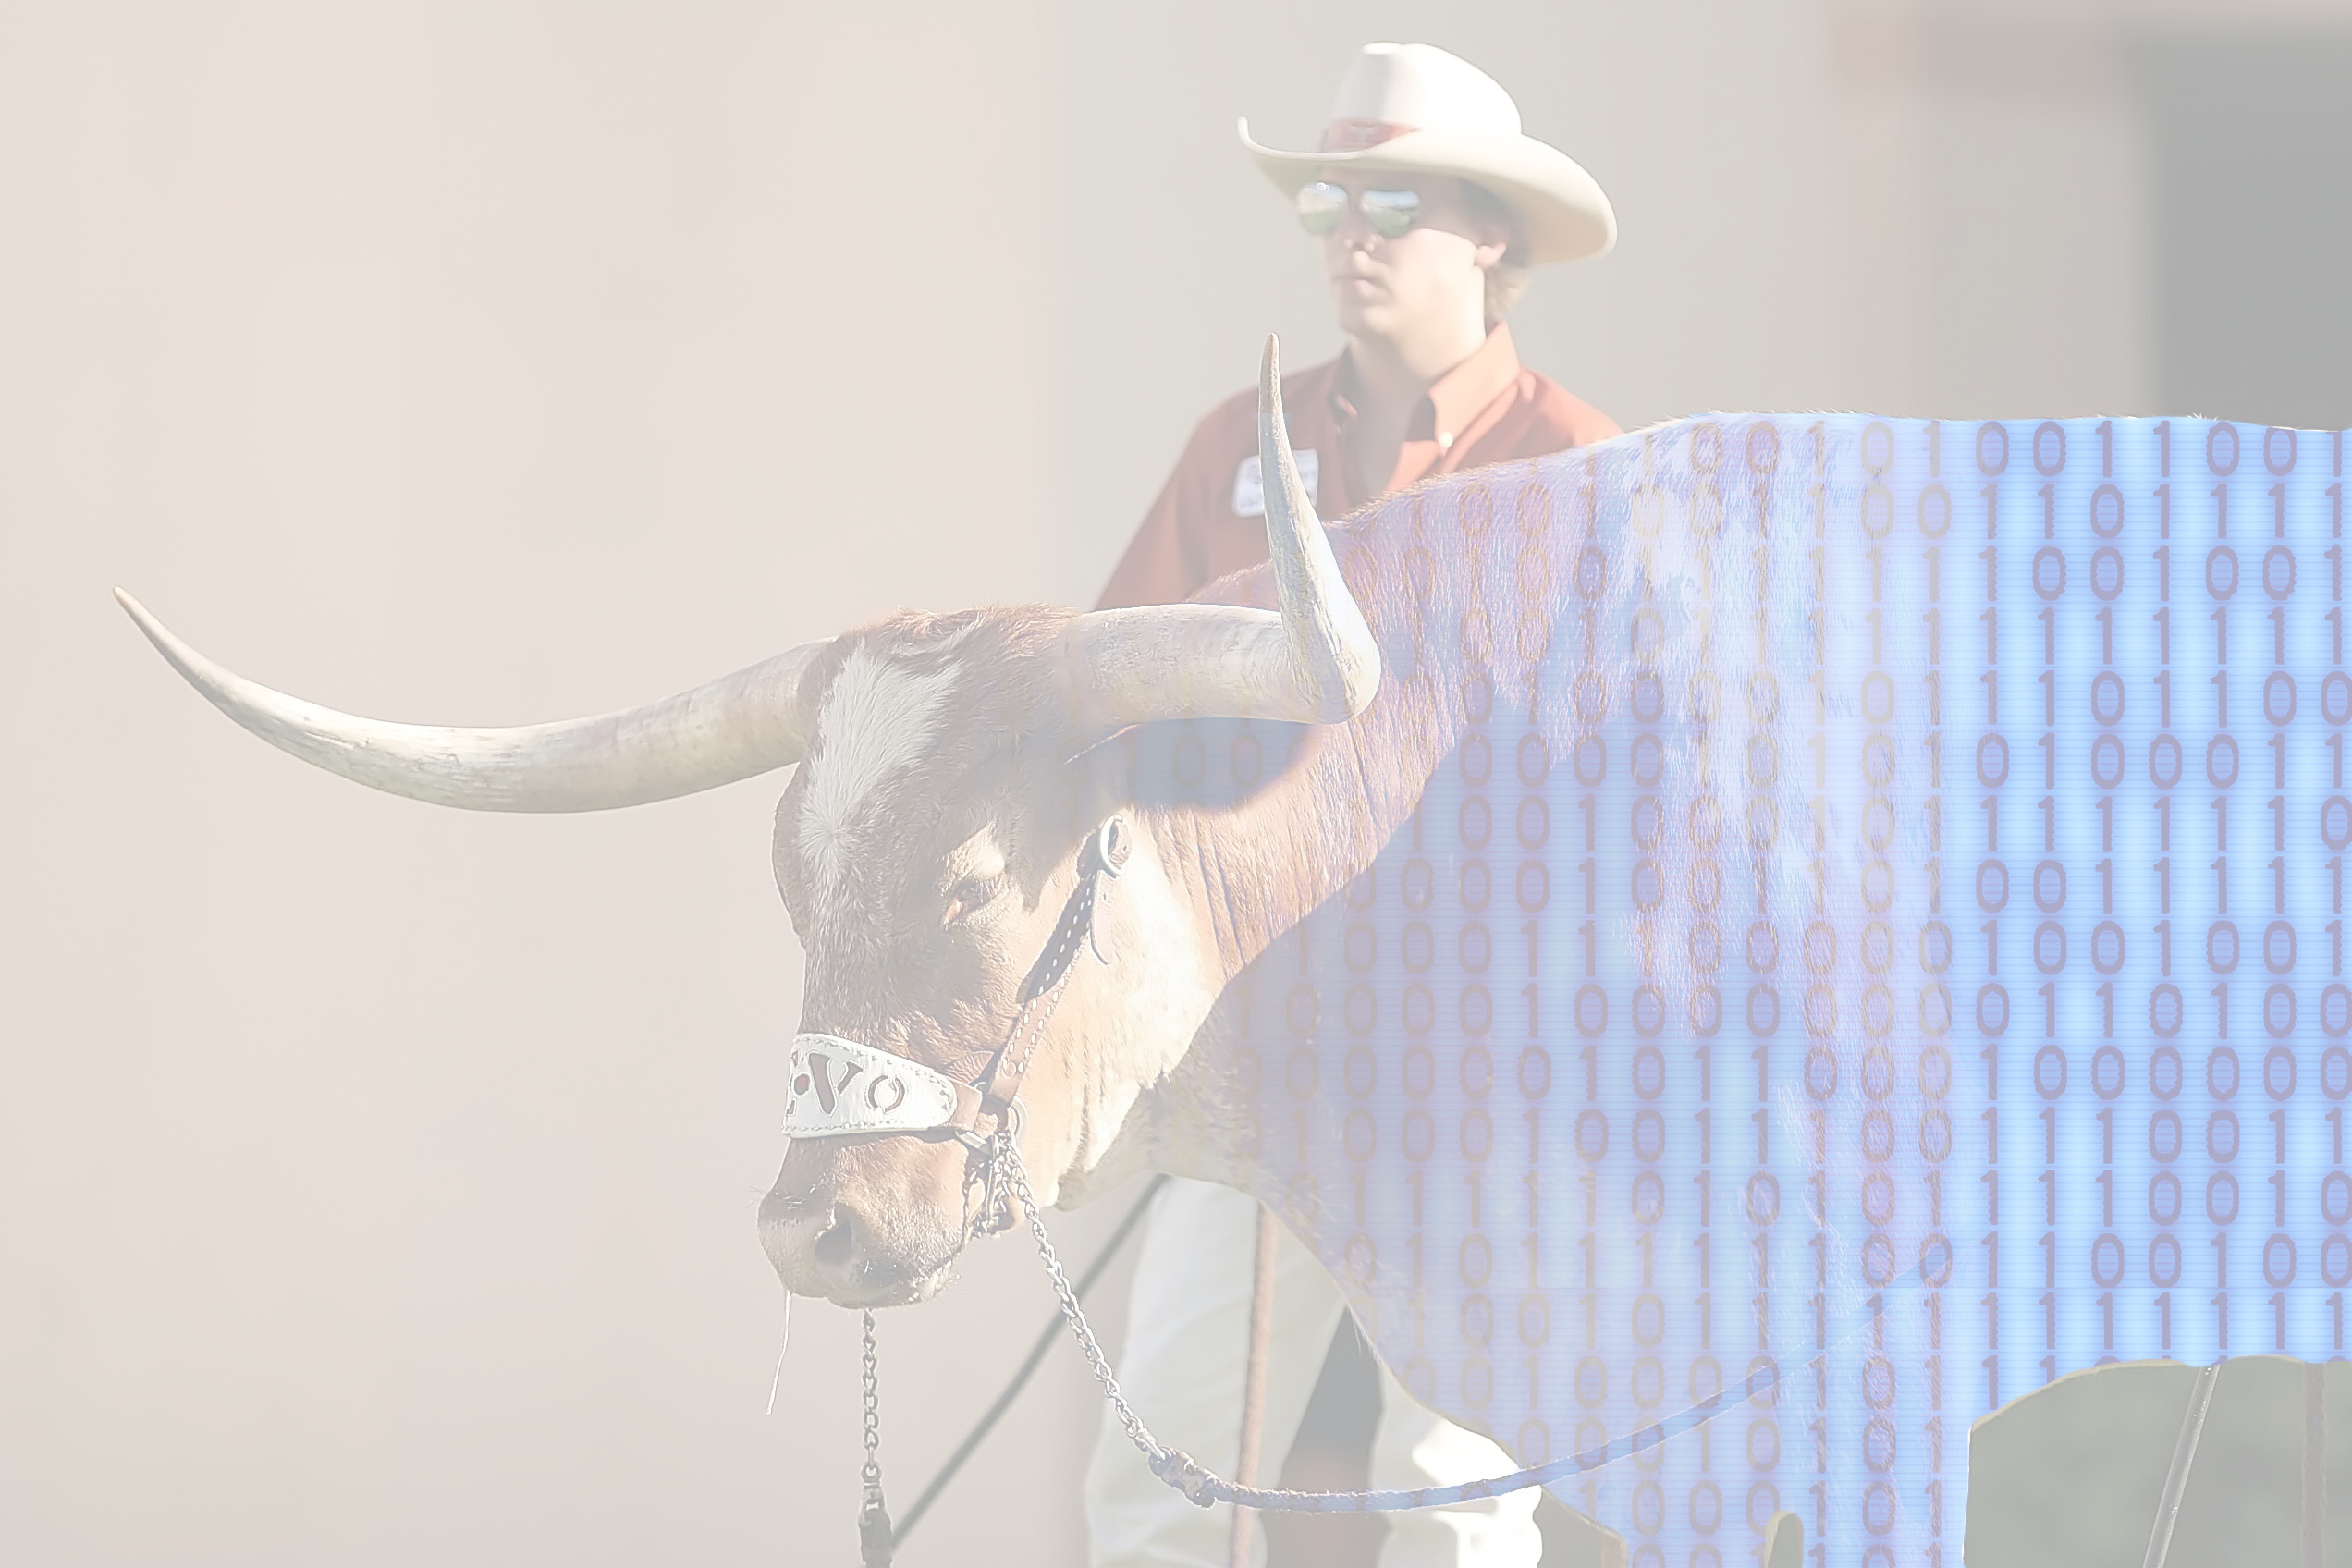
\includegraphics[height=\paperheight,keepaspectratio]{data-wrangler-BG.jpg}}
% to create image:
%   1. export data-wrangler.xcf as PNG from GIMP
%   2. convert data-wrangler.png -fill white -colorize 67% data-wrangler-BG.jpg

\begin{frame}
    \thispagestyle{empty}
    \titlepage
\end{frame}

\setbeamertemplate{background canvas}[default]


%%%%%%%%%%%%%%%%%%%%%%%%%%%%%%%%%%%%%%%%%%%%%%%%%%%%%%%%%%%%%%%%%%%%%%%%%%%%%%%%


\begin{frame}<beamer>
    \thispagestyle{empty}
    \begin{tikzpicture}[remember picture, overlay]
        \only<1>{
            \node (picture) at (current page.center) {
                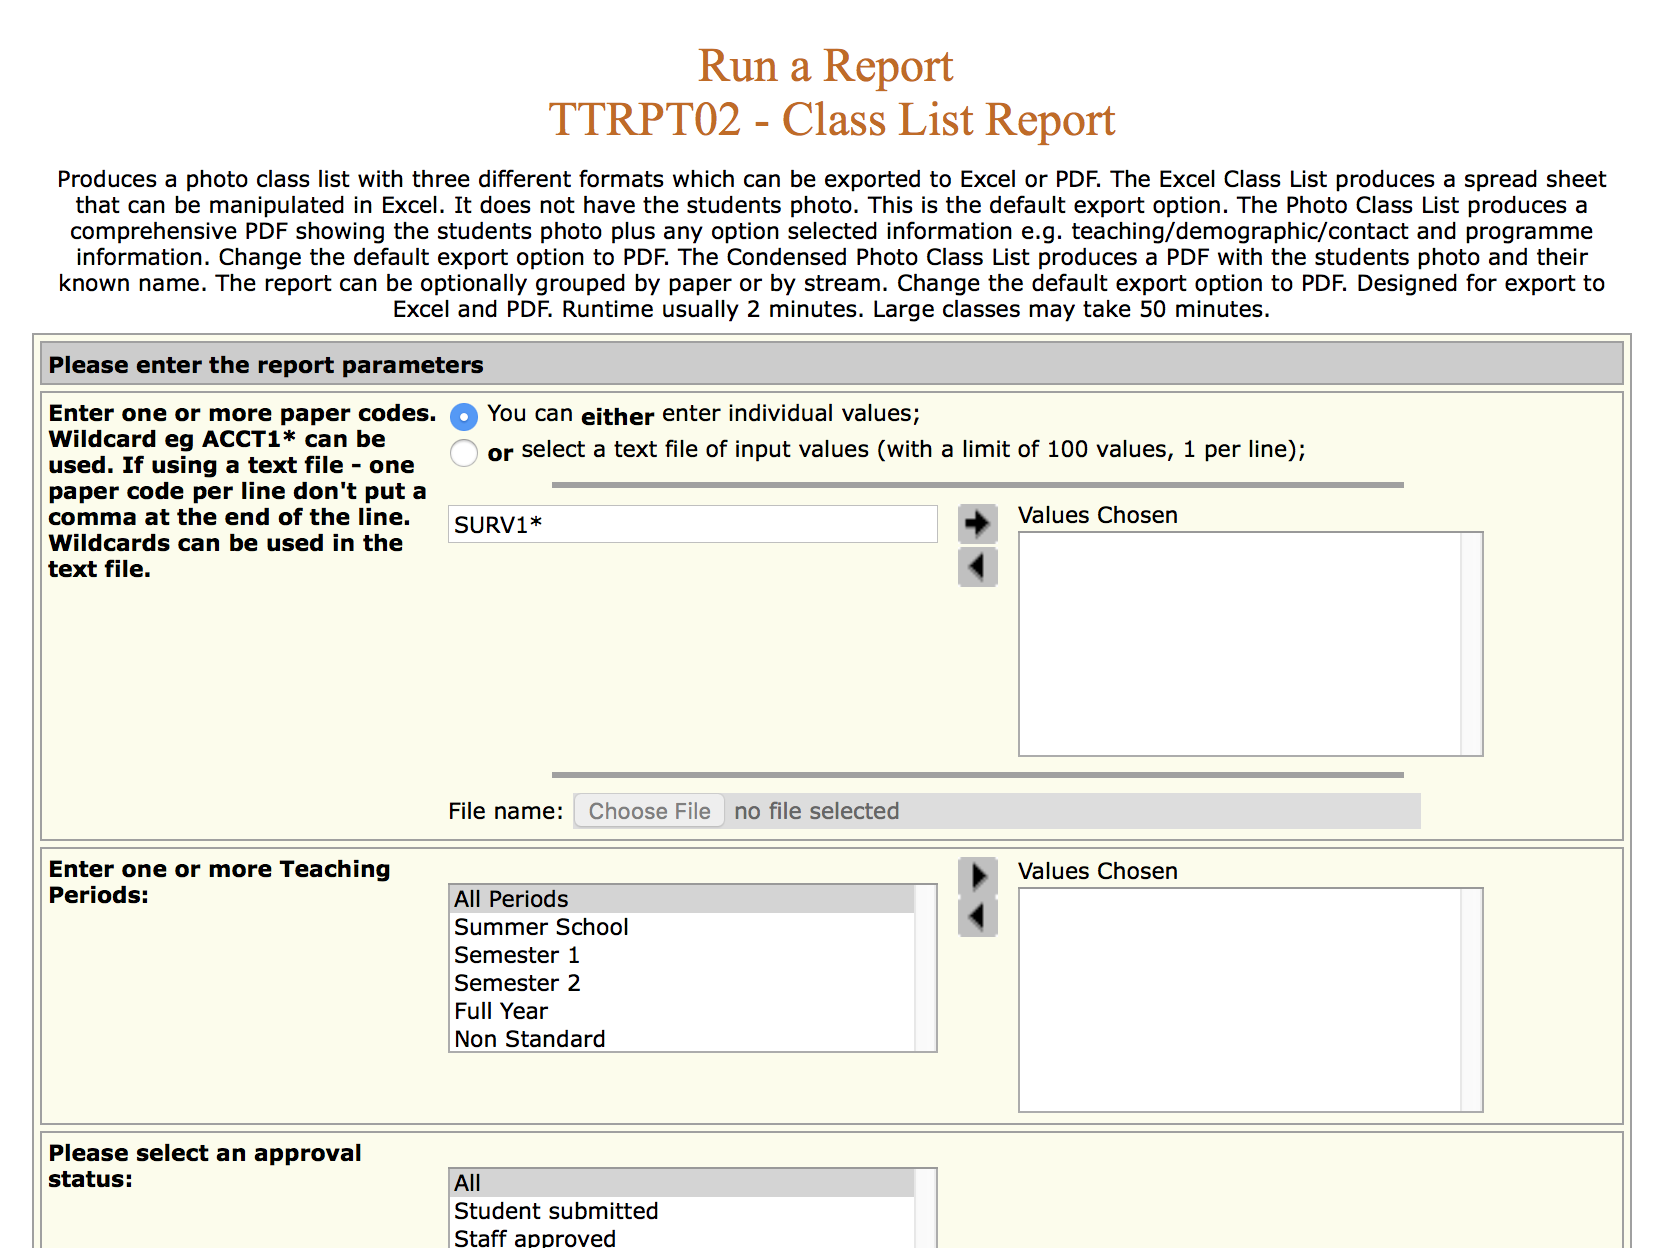
\includegraphics[width=\paperwidth,keepaspectratio]{TTRPT02.png}
            };
            \node[anchor=north west] (logo) at (current page.north west) {
                
\includegraphics[width=3.5cm,keepaspectratio,angle=10]{BO.png}
            };
        }
    \end{tikzpicture}
    \only<2>{\mbox{}}
\end{frame}


%%%%%%%%%%%%%%%%%%%%%%%%%%%%%%%%%%%%%%%%%%%%%%%%%%%%%%%%%%%%%%%%%%%%%%%%%%%%%%%%


\begin{frame}
    \frametitle{Data come from a \uline{lot} of different sources}
    
    \bigskip
    \begin{columns}
        \begin{column}{0.4\paperwidth}
            \centering
            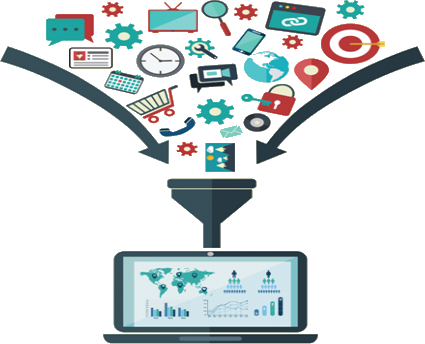
\includegraphics[width=0.9\columnwidth,keepaspectratio]{data-sources.png}\tinyskip
            {\tiny{SOURCE: Xobber}}
        \end{column}
        \begin{column}{0.55\paperwidth}
            \centering
            \begin{tabular}{cccccccc}
                \faHeartO & \faCode & \faDatabase & \faGit & \faCalendar & \faLaptop & \faThumbsOUp & \faBluetoothB \\
                \addlinespace
                \faTags & \faTerminal & \faDashboard & \faYoutubePlay & \faFileCodeO & \faLinux & \faCloud & \faBank \\
                \addlinespace
                \faBarcode & \faUsers & \faFilePdfO & \faSafari & \faAndroid & \faAmazon & \faFileAudioO & \faGavel \\
                \addlinespace
                \faFileWordO & \faFilm & \faRss & \faSteam & \faWikipediaW & \faCreditCard & \faGamepad & \faWifi \\
                \addlinespace
                \faShoppingCart & \faPaypal & \faKeyboardO & \faClockO & \faEnvelopeO & \faFileExcelO & \faTruck & \faToggleOn \\
                \addlinespace
                \faBirthdayCake & \faFolderOpenO & \faHddO & \faDesktop & \faAutomobile & \faBus & \faResistance & \faFax \\
                \addlinespace
                \faGoogle & \faFacebook & \faIndustry & \faLinkedin & \faAreaChart & \faSpotify & \faBarChart & \faFileTextO \\
                \addlinespace
                \faFloppyO & \faWeibo & \faFileArchiveO & \faFileImageO & \faPrint & \faMobile & \faApple & \faChrome \\
                \addlinespace
                \faPieChart & \faCamera & \faQrcode & \faSoccerBallO & \faMapO & \faFirefox & \faFilePowerpointO & \faEdge \\
                \addlinespace
                \faCompass & \faNewspaperO & \faFileMovieO & \faStackOverflow & \faMicrophone & \faTwitter & \faWpforms & \faPhone \\
            \end{tabular}
        \end{column}
    \end{columns}
\end{frame}


%%%%%%%%%%%%%%%%%%%%%%%%%%%%%%%%%%%%%%%%%%%%%%%%%%%%%%%%%%%%%%%%%%%%%%%%%%%%%%%%


\begin{frame}
    \frametitle{Data schemas run a wide gamut}
    
    \begin{columns}
        \begin{column}{\paperwidth}
            \centering
            \begin{tikzpicture}
                \node (erd) {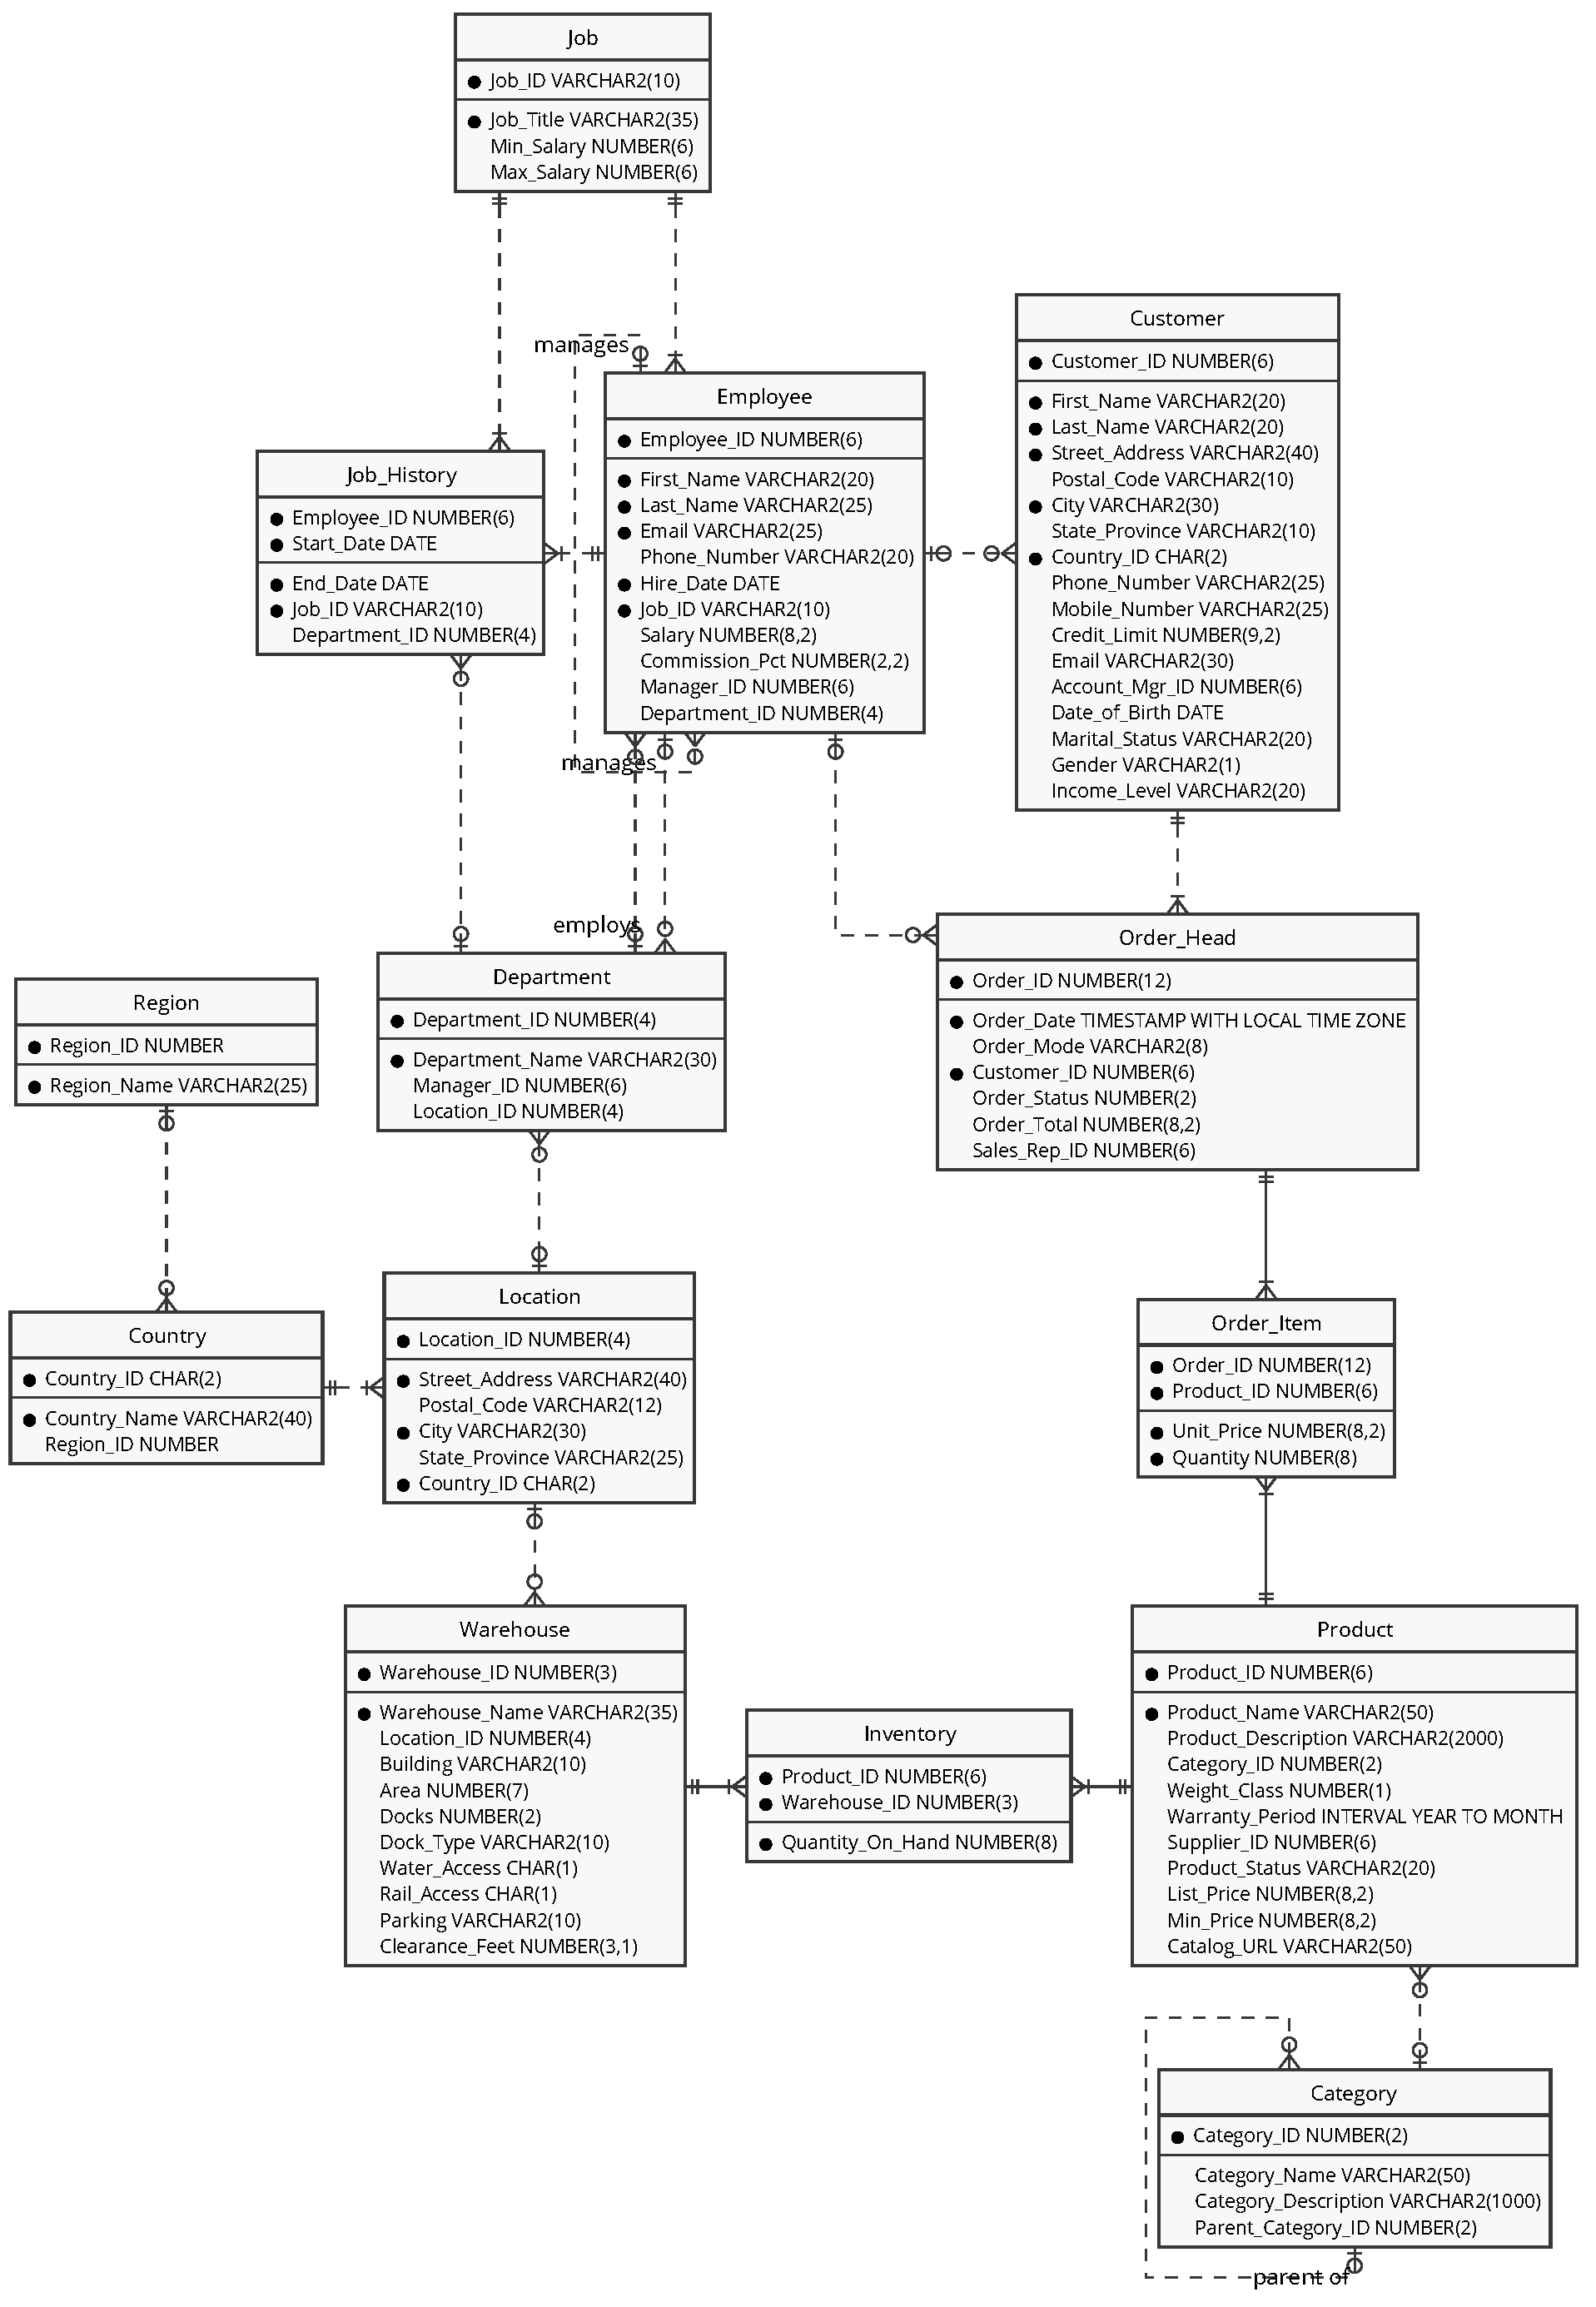
\includegraphics[width=3.25cm,keepaspectratio]{HR_OE_ERD}};
                \node[right=7.5mm of erd] (excel) {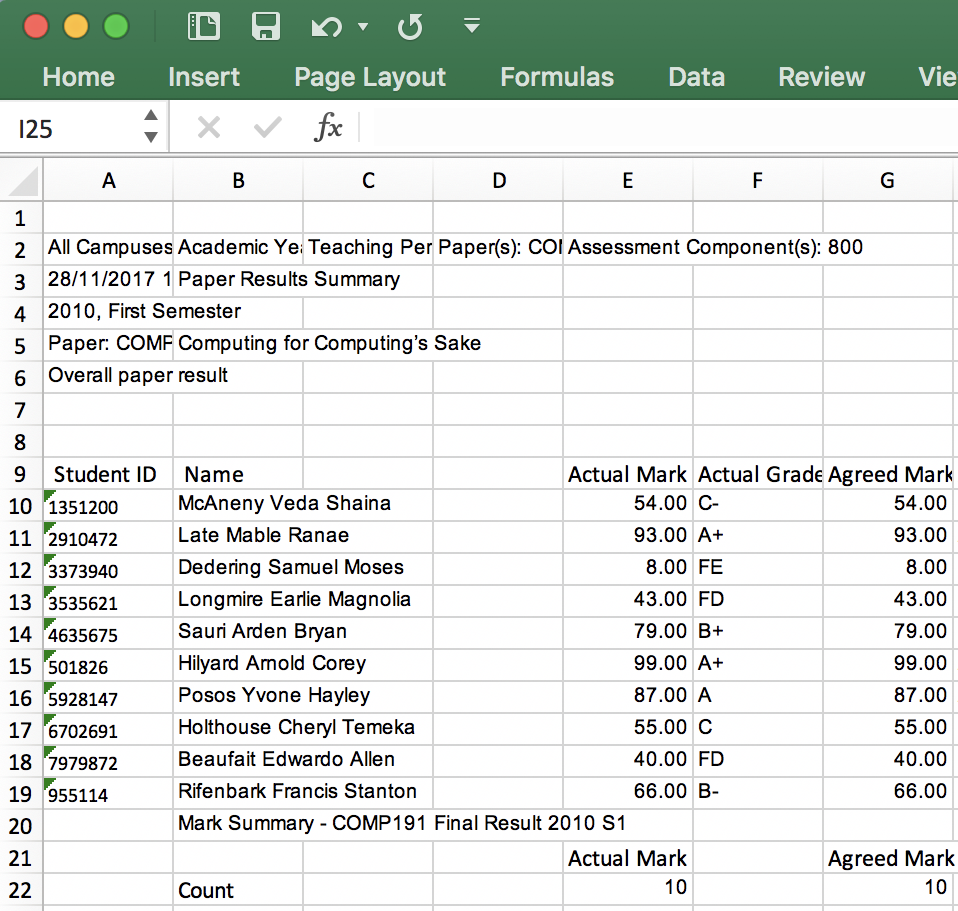
\includegraphics[width=3.25cm,keepaspectratio]{fake_results_excel}};
                \node[right=7.5mm of excel] (web) {
\includegraphics[width=3.25cm,keepaspectratio]{web_page}};
                
                \node[below=0mm of web.south] (weblabel) {free-form};
                \node (excellabel) at (excel |- weblabel) {more flexible};
                \node (erdlabel) at (erd |- weblabel) {formal, “fixed”};
                
                \node[below=-3pt of erdlabel] (erdtext) {\tiny e.g., SQL databases};
                \node[below=-3pt of excellabel] (exceltext) {\tiny e.g., JSON, XML, Excel, …};
                \node[below=-3pt of weblabel] (webtext) {\tiny e.g., email, MS Word, web pages, …};
                
                \path[fill, OU red, ultra thick, nearly transparent] (erd.west) -- ++(0,1cm) -- ($(web.west) + (0,1cm)$) -- ++(0,1cm) -- (web.east) -- ($(web.west) - (0,2cm)$) -- ++(0,1cm) -- ($(erd.west) - (0,1cm)$) -- cycle;
            \end{tikzpicture}
        \end{column}
    \end{columns}
\end{frame}


%%%%%%%%%%%%%%%%%%%%%%%%%%%%%%%%%%%%%%%%%%%%%%%%%%%%%%%%%%%%%%%%%%%%%%%%%%%%%%%%


\begin{frame}
    \frametitle{Moving data around can lead to … trouble}
    
    \bigskip
    \centering
    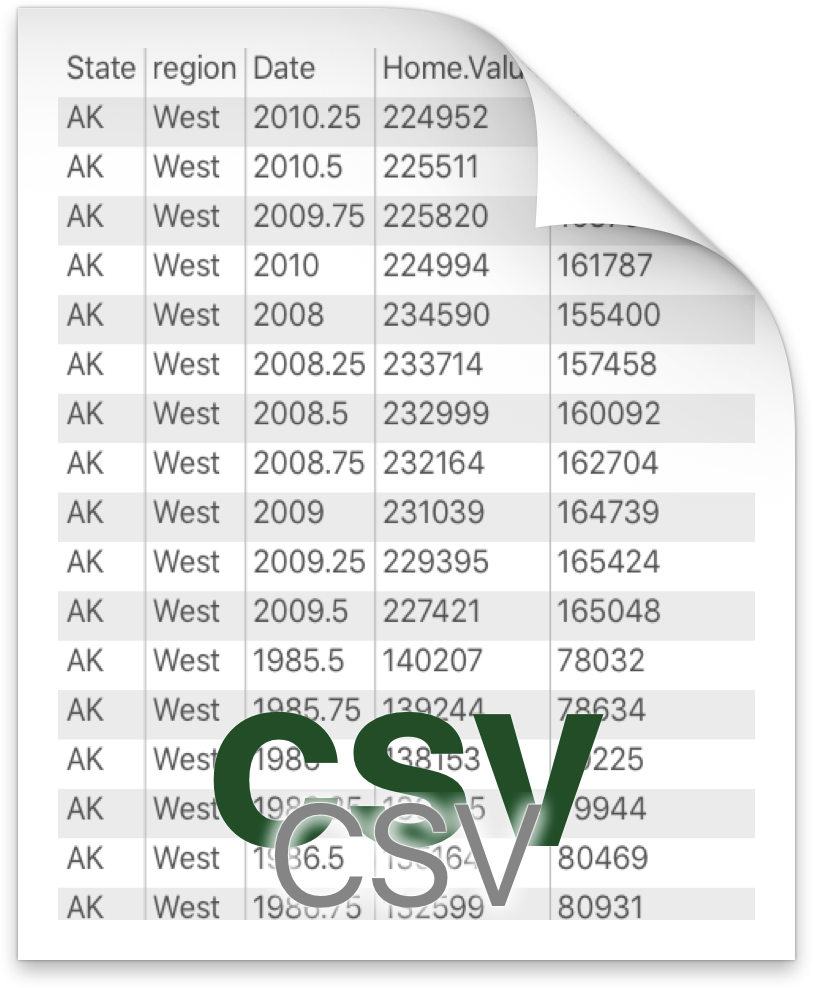
\includegraphics[height=6cm,keepaspectratio]{CSV}
    
    \begin{tikzpicture}[remember picture, overlay]
        \node[below right=1cm of current page.west] (ed209) {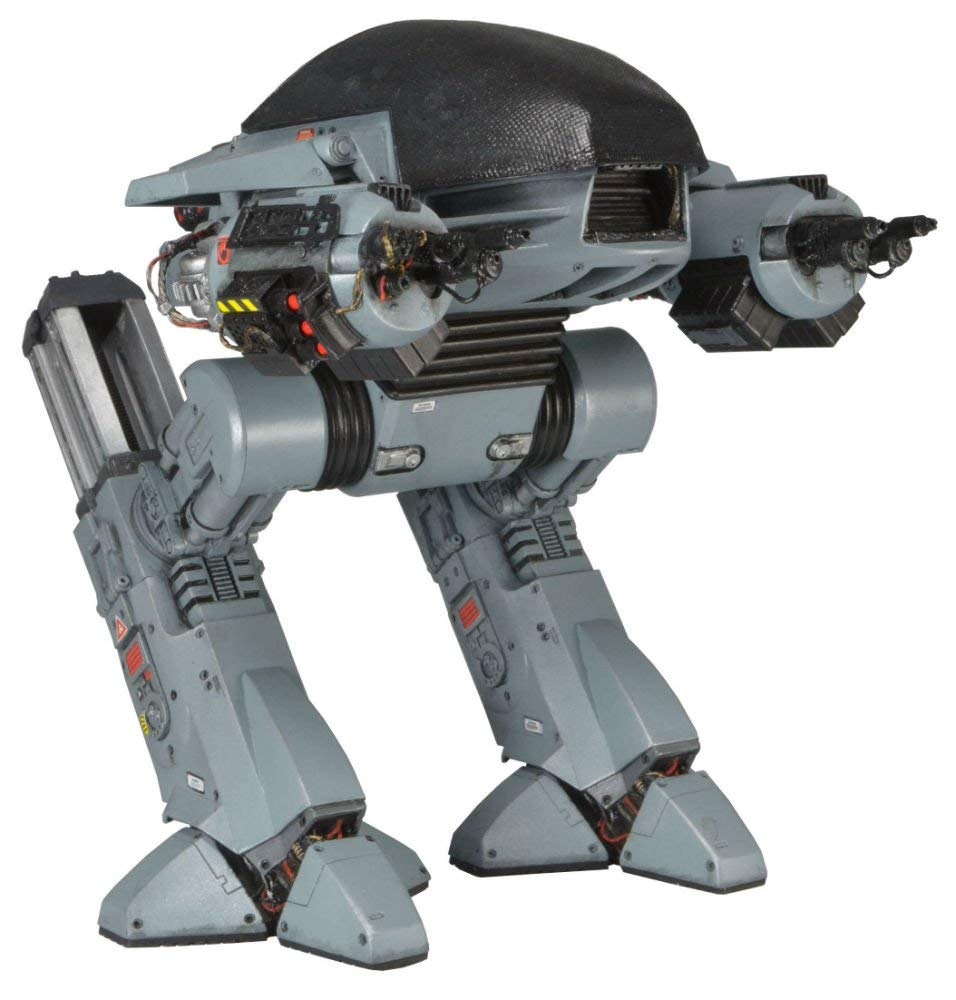
\includegraphics[width=2cm,keepaspectratio]{ED-209}};
    \end{tikzpicture}
\end{frame}


%%%%%%%%%%%%%%%%%%%%%%%%%%%%%%%%%%%%%%%%%%%%%%%%%%%%%%%%%%%%%%%%%%%%%%%%%%%%%%%%


\begin{frame}
    \huge
    \centering
    \bigskip\bigskip
    \structurebf{Often it’s not a case of what we can get from the data, but rather what data \emph{can} we get?}
\end{frame}


%%%%%%%%%%%%%%%%%%%%%%%%%%%%%%%%%%%%%%%%%%%%%%%%%%%%%%%%%%%%%%%%%%%%%%%%%%%%%%%%


\begin{frame}
    \frametitle{Project 1: CoreScan (completed)}
    
    \bigskip
    \begin{itemize}
        \item Statistical analysis of body composition data in R to check precision of GE’s new CoreScan algorithm. {\tiny (densitometry)}
        
        \item Data exported directly from DXA body scanner. {\tiny (dual X-ray absorptiometry)}
        
        \item Relatively straightforward:
        \begin{itemize}
            \item Excel with well-defined columns
            \item some minor cleaning
            \item trivial to automate
        \end{itemize}
        
        \item “The way things should be.”
    \end{itemize}
    
    \begin{tikzpicture}[remember picture, overlay]
        \node[above right=5mm of current page.south west)] (ref) {
            \scriptsize\parbox{\columnwidth}{Meredith-Jones, K., Haszard, J., Stanger, N., and Taylor, R. “Precision of DXA-derived visceral fat measurements in a large sample of adults of varying body size.” \emph{Obesity} \textbf{26}(3):505–512. doi:~10.1002/oby.22108}
        };
    \end{tikzpicture}
\end{frame}


%%%%%%%%%%%%%%%%%%%%%%%%%%%%%%%%%%%%%%%%%%%%%%%%%%%%%%%%%%%%%%%%%%%%%%%%%%%%%%%%


\setbeamertemplate{background canvas}{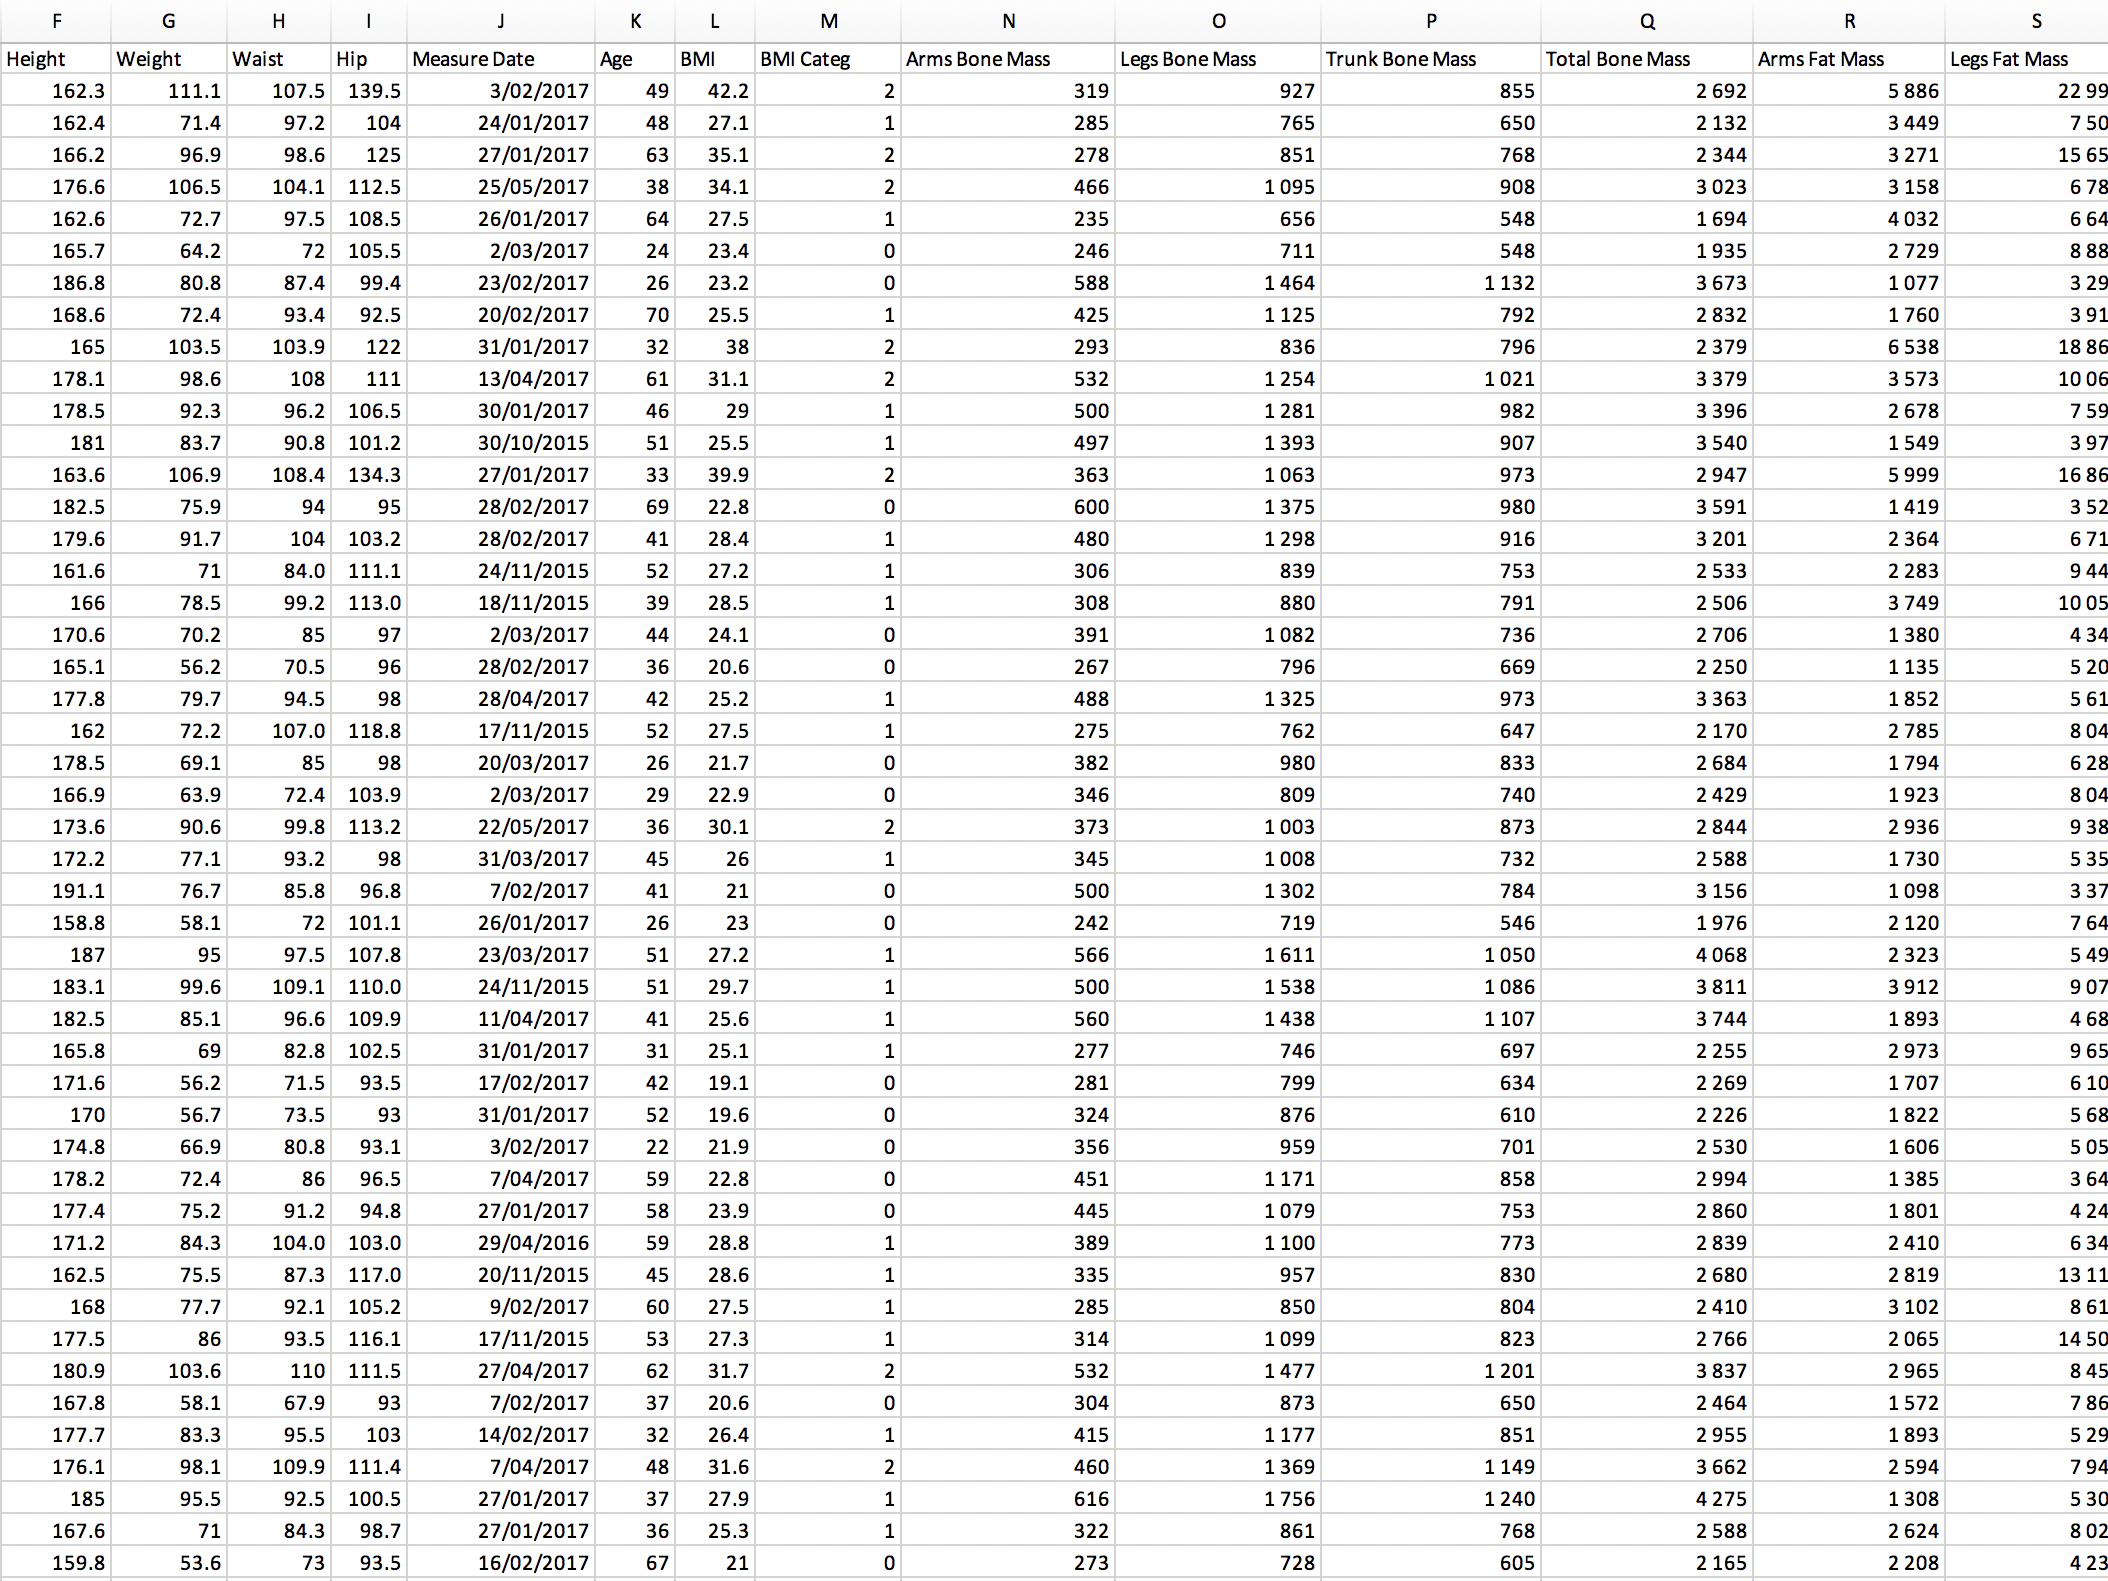
\includegraphics[width=\paperwidth,keepaspectratio]{CoreScan_data.png}}

\begin{frame}
    \thispagestyle{empty}
\end{frame}

\setbeamertemplate{background canvas}[default]


%%%%%%%%%%%%%%%%%%%%%%%%%%%%%%%%%%%%%%%%%%%%%%%%%%%%%%%%%%%%%%%%%%%%%%%%%%%%%%%%


\newcommand\redstrike{\bgroup\markoverwith
      {\textcolor{red}{\rule[0.45ex]{2pt}{1.5pt}}}\ULon}
      
\begin{frame}
    \frametitle{Project 2: Software licensing (barely started)}
    
    \structurebf{Which is cheaper for consumer-level software, subscription or perpetual licensing?}
    \medskip
    
    \begin{itemize}
        \item SaaS already well studied, especially for corporates.
        
        \item Typical licensing models for smaller developers:
        \begin{itemize}
            \item pay once, all updates free forever
            \item pay for each major version upgrade {\tiny (upgrade pricing)}
            \item app store (free or paid) + in-app purchases
        \end{itemize}

        \item Some are experimenting with alternative models:
        \begin{itemize}
            \item “service contract” (e.g., annual subscription)
            \item “software plus a service” (\redstrike{SpaS?} \alert{\textbf{NO}} S+aS? S++S?)
        \end{itemize}
        
        \item Some developers offer more than one of these options.
    \end{itemize}
\end{frame}


%%%%%%%%%%%%%%%%%%%%%%%%%%%%%%%%%%%%%%%%%%%%%%%%%%%%%%%%%%%%%%%%%%%%%%%%%%%%%%%%


\begin{frame}
    \frametitle{Why do I care?}
    
    \structurebf{1Password now offers two licensing models:}
    \medskip
    
    \begin{itemize}
        \item Typical perpetual license:
        \begin{itemize}
            \item separate licenses per platform {\tiny (to enable \emph{all} features)}
            \item manually configured syncing
            \item major version upgrades are (usually) paid
            \item “pro” mobile apps are one-off in-app purchase
        \end{itemize}
        
        \item Subscription:
        \begin{itemize}
            \item free license for all platform apps
            \item transparent syncing via 1Password account
            \item annual vs.\ monthly billing
            \item individual vs.\ family {\tiny (additional group features)}
        \end{itemize}
        
        \item Both options via direct sale or app store.
    \end{itemize}
    
    \medskip
    \centering
    \alert{\fbox{\textbf{Which version should I buy?}}}
    
    \begin{tikzpicture}[remember picture, overlay]
        \node[below left=1.25cm of current page.north east)] (icon) {
            
\includegraphics[width=2cm,keepaspectratio]{1Password}
        };
    \end{tikzpicture}
\end{frame}


%%%%%%%%%%%%%%%%%%%%%%%%%%%%%%%%%%%%%%%%%%%%%%%%%%%%%%%%%%%%%%%%%%%%%%%%%%%%%%%%


\begin{frame}
    \frametitle{Cost comparison (US\$)}
    \framesubtitle{(based on my purchase records)}
    
    \begin{columns}[t]
        \begin{column}{0.4\paperwidth}
            \structurebf{“Standard” license}
            \bigskip
            
            \begin{tabular}{rrr}
                \textbf{Version}    &   \textbf{When}   &   \textbf{Cost}\textcolor{white}{*} \\
                2, 3 (4?)           &   Feb 2009        &   \$39.95\textcolor{white}{*}   \\
                5, 6                &   Dec 2014        &   \$24.99\textcolor{white}{*}   \\
                7                   &   Jun 2018        &   \$49.99*   \\
                iOS                 &   N/A             &   \$9.99\textcolor{white}{*}  \\
                \addlinespace
                \multicolumn{3}{r}{Total (≈\,113 months): \$124.92\textcolor{white}{*}}   \\
                \multicolumn{3}{r}{Total (per month): ≈\,\$1.11\textcolor{white}{*}}   \\
                \multicolumn{3}{r}{\alert{Total (per year): ≈\,\$13.27}\textcolor{white}{*}}   \\
                \addlinespace
                \multicolumn{3}{l}{\tiny *\,introductory price; normally \$64.99 \(\Rightarrow\) \$14.86 per year}
            \end{tabular}
        \end{column}
        \begin{column}{0.4\paperwidth}
            \quad\structurebf{Subscription}
            \begin{tabbing}
                \quad Individual \= = \$2.99 per month \\
                \> = \$35.88 per year \\[6pt]
                \quad Family \= = \$4.99 per month \\
                \> = \$59.88 per year \\
                \\
                \quad \structurebf{Are the extra features really} \\
                \quad \structurebf{worth \emph{that} much?}
            \end{tabbing}
        \end{column}
    \end{columns}
\end{frame}


%%%%%%%%%%%%%%%%%%%%%%%%%%%%%%%%%%%%%%%%%%%%%%%%%%%%%%%%%%%%%%%%%%%%%%%%%%%%%%%%


\begin{frame}
    \frametitle{The data collection problem}
    
    \structurebf{To compare costs we need historical pricing}
    \medskip
    
    \begin{itemize}
        \item No-one’s likely to publish their pricing history! {\tiny (who cares?)}
        \begin{itemize}
            \item except maybe vendors that sell separate versions for different OS releases {\tiny (e.g. macOS Mail plugins)}
            \item at best probably only full pricing available, not upgrade
        \end{itemize}
        
        \item Wayback Machine? {\tiny (Internet Archive)}
        \begin{itemize}
            \item I have found a couple of old store-fronts
            \item probably impossible to automate \faFrownO
        \end{itemize}
        
        \item Trivial to process, but effectively worst case to acquire.
        
        \item Watch this space!
    \end{itemize}
\end{frame}


%%%%%%%%%%%%%%%%%%%%%%%%%%%%%%%%%%%%%%%%%%%%%%%%%%%%%%%%%%%%%%%%%%%%%%%%%%%%%%%%


\begin{frame}
    \frametitle{“Project” 3: Student data (ongoing)}
    
    \begin{itemize}
        \item For teaching \& administration:
        \begin{itemize}
            \item class lists
            \item email lists
            \item internal assessment {\tiny (ISPMS)}
            \item terms
            \item timetabling
            \item \alert<2>{final results {\tiny (INFORMS)}}
        \end{itemize}
        
        \item For research:
        \begin{itemize}
            \item \alert<2>{CALT project on data driven course advising {\tiny (UCAN)}}
            \item efficacy of teaching/tool interventions
            \item …
        \end{itemize}
    \end{itemize}
\end{frame}


%%%%%%%%%%%%%%%%%%%%%%%%%%%%%%%%%%%%%%%%%%%%%%%%%%%%%%%%%%%%%%%%%%%%%%%%%%%%%%%%


\begin{frame}
    \frametitle{INFORMS}
    \framesubtitle{(also ISPMS to some extent)}
    
    \begin{itemize}
        \item Initially a PostgreSQL database + tools to automatically generate results files for Student Records. {\tiny (ca.\ 2001–2002)}
        
        \item Has grown “organically”:
        \begin{itemize}
            \item transforming data to and from central systems {\tiny (pre and post eVision)}
            \item level of award calculation
            \item grade histograms and other statistics
            \item automated result proofing
            \item web interface for some functions
            \item[\faArrowRight] a mishmash of bash, Perl, Python, PHP, R, AppleScript (!), iMacros, HTML, CSS, JavaScript
        \end{itemize}
    \end{itemize}
    \bigskip\bigskip\bigskip\bigskip\mbox{}
    
    \begin{tikzpicture}[remember picture, overlay]
        \node[anchor=south west, above right=3.5mm of current page.south west] (home) {
            
\includegraphics[height=3cm,keepaspectratio]{INFORMS_home}
        };
        \node[anchor=south east, above left=3.5mm of current page.south east] (files) {
            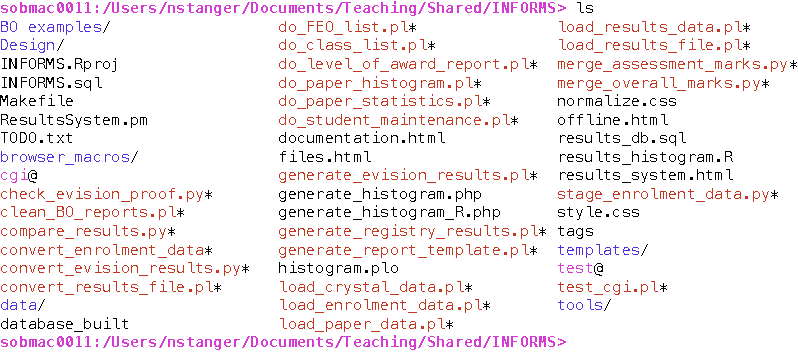
\includegraphics[height=3cm,keepaspectratio]{INFORMS_files}
        };
    \end{tikzpicture}
\end{frame}


%%%%%%%%%%%%%%%%%%%%%%%%%%%%%%%%%%%%%%%%%%%%%%%%%%%%%%%%%%%%%%%%%%%%%%%%%%%%%%%%


\begin{frame}
    \frametitle{Data driven course advising}
    \framesubtitle{(with Sander, Claudia, Steven, and others since Jan 2018)}
    
    \begin{itemize}
        \item CALT project looking at evidence-based approaches to improve course advising. {\tiny (among other things)}
        
        \item Needs widely varied historical student data.
        \begin{itemize}
            \item enrolments, results, student performance, workload, degree completion, demographics, …
            \item initially focused on COSC and INFO papers only
        \end{itemize}
        
        \item Raw data set 2009–2018 (S1):
        \begin{itemize}
            \item 9743 students, 578 offerings of 110 papers, \num{29238} enrolments
            \item ≈\,60\% enrolled in computing majors, ≈\,16\% in computing minors
            \item using modified version of INFORMS database
        \end{itemize}
    \end{itemize}
\end{frame}


%%%%%%%%%%%%%%%%%%%%%%%%%%%%%%%%%%%%%%%%%%%%%%%%%%%%%%%%%%%%%%%%%%%%%%%%%%%%%%%%


\begin{frame}
    \frametitle{Visualisation: Student flows between papers}
    
    \begin{columns}[t]
        \begin{column}{0.5\paperwidth}
            \centering
            \structurebf{Something like this would be great}
            \medskip
            
            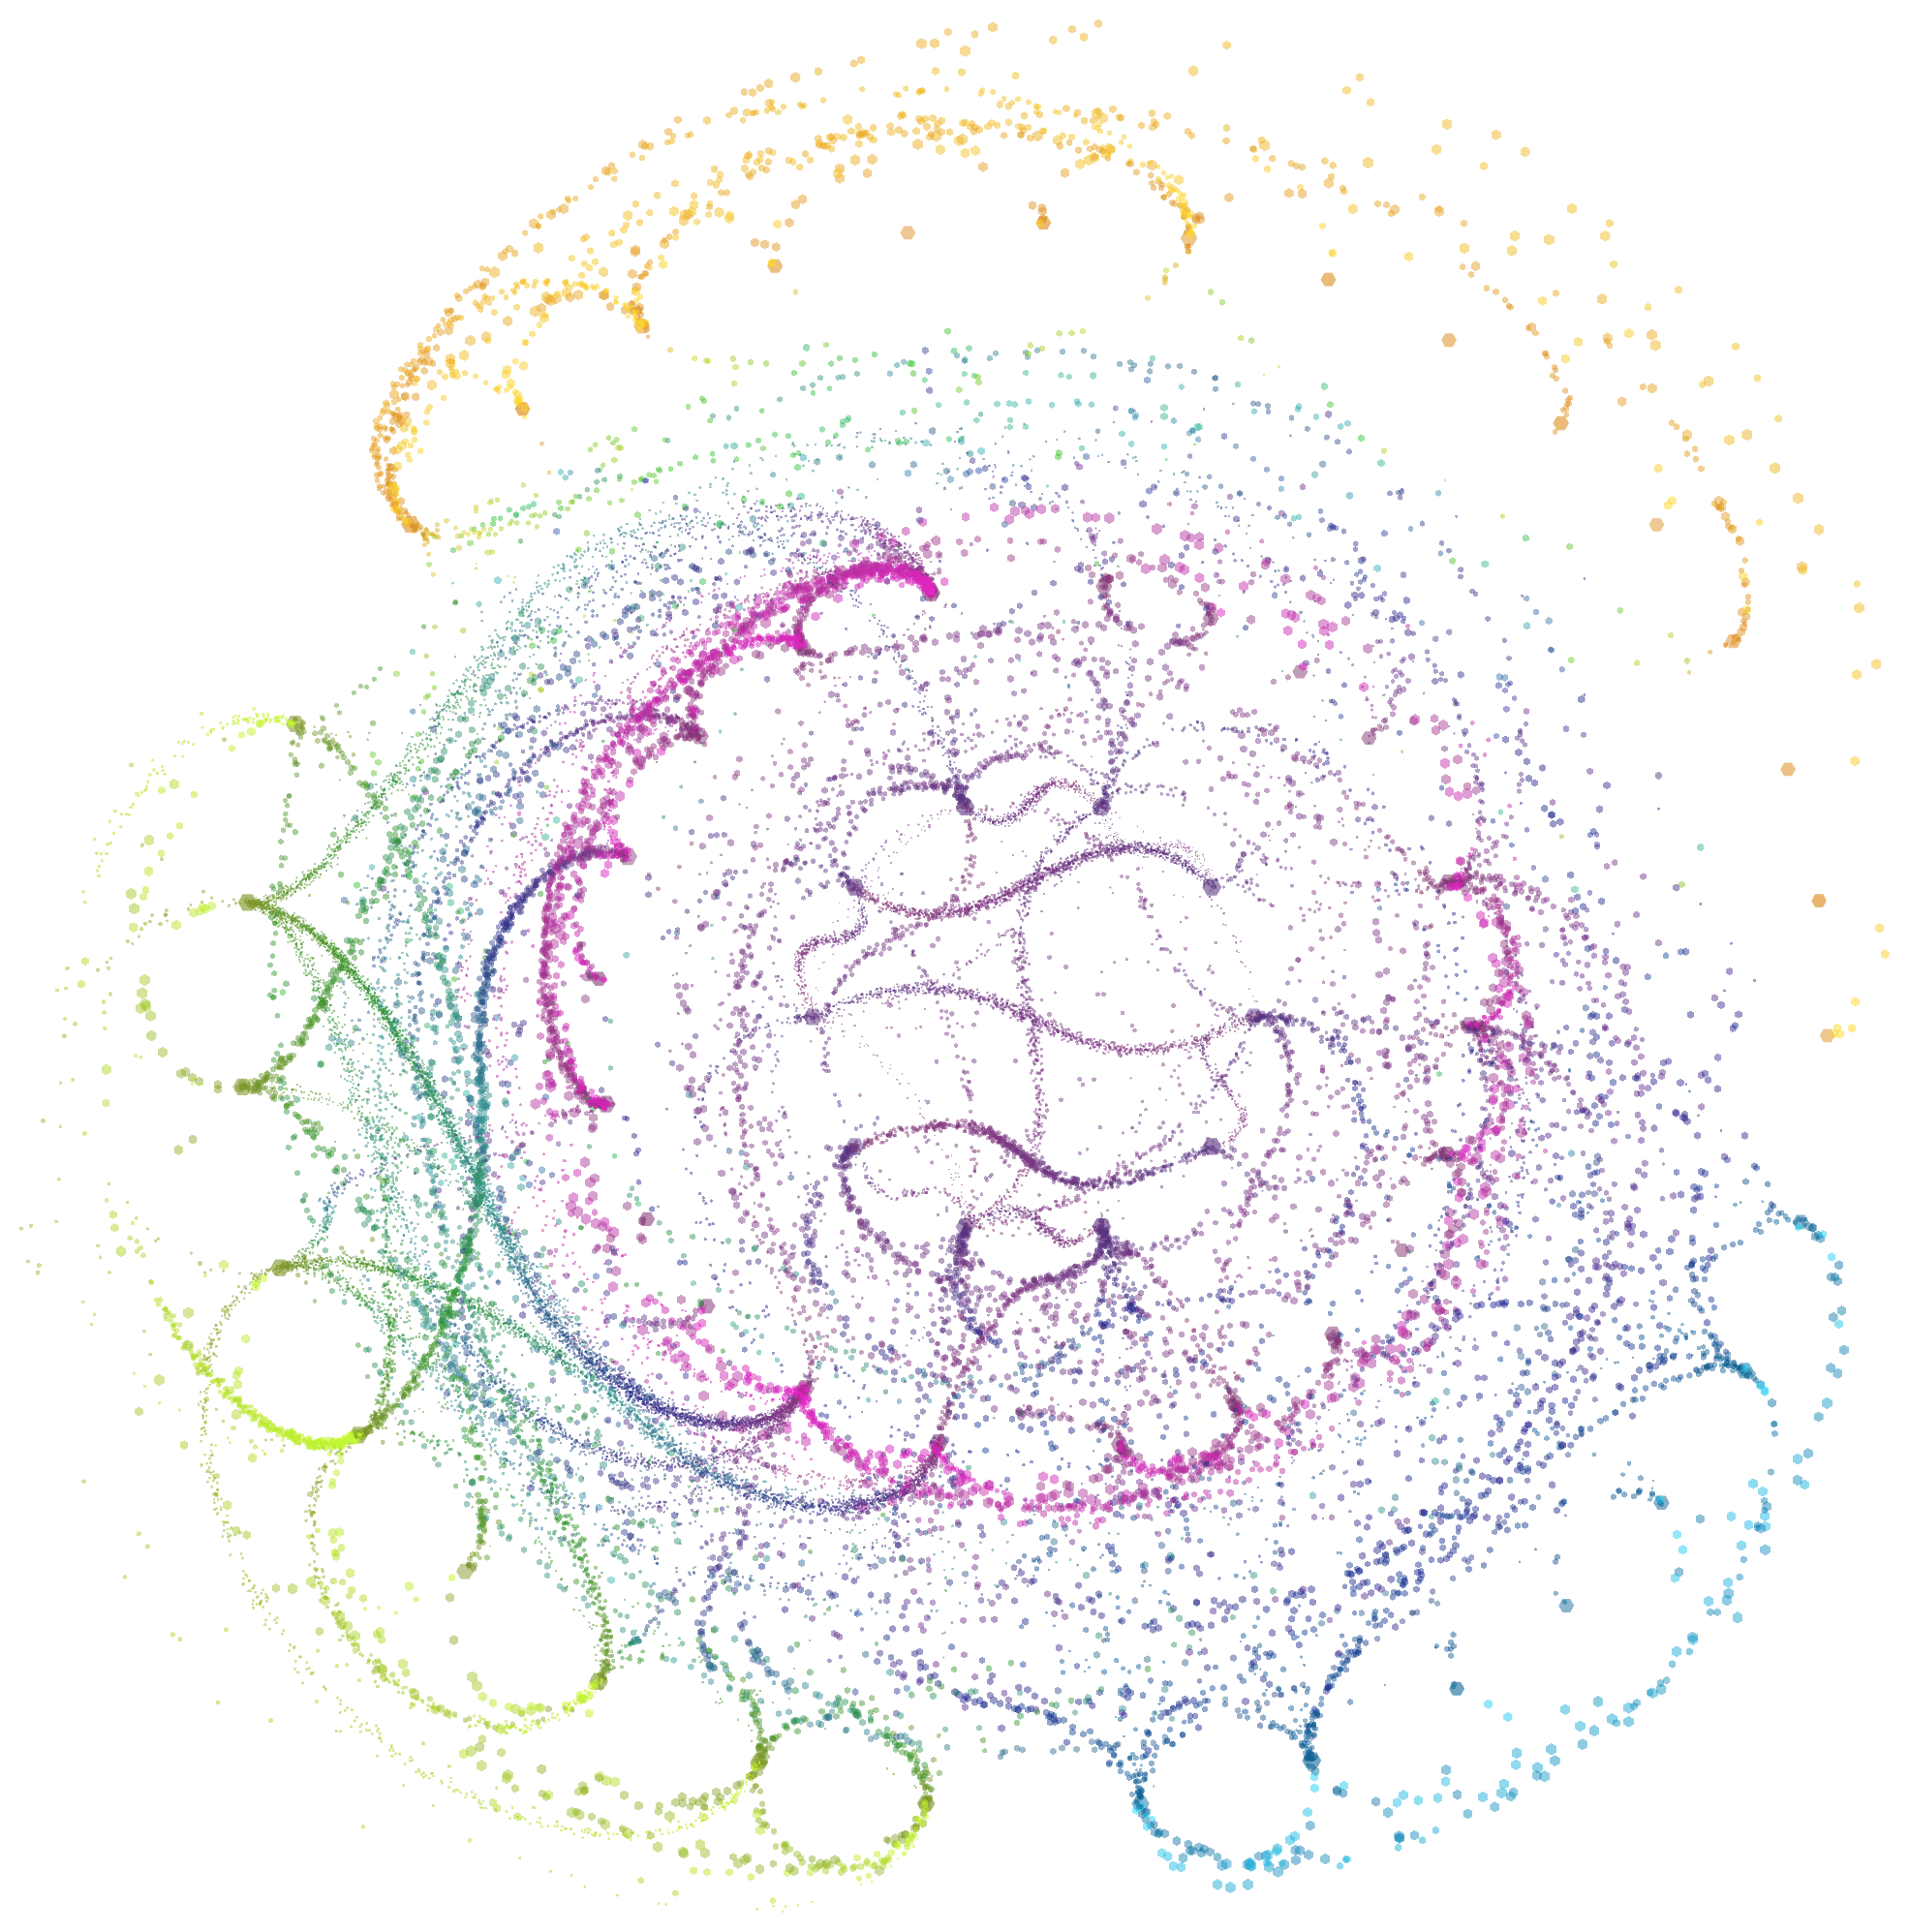
\includegraphics[width=0.8\columnwidth,keepaspectratio]{AthenaHealth.png}\tinyskip
            {\tiny SOURCE: \href{http://athenahealthvisualization.com}{Fathom/Athena Health}}
        \end{column}
        \begin{column}{0.5\paperwidth}
            \centering
            \structurebf{But we still need a bit of work…}
            \medskip
            
            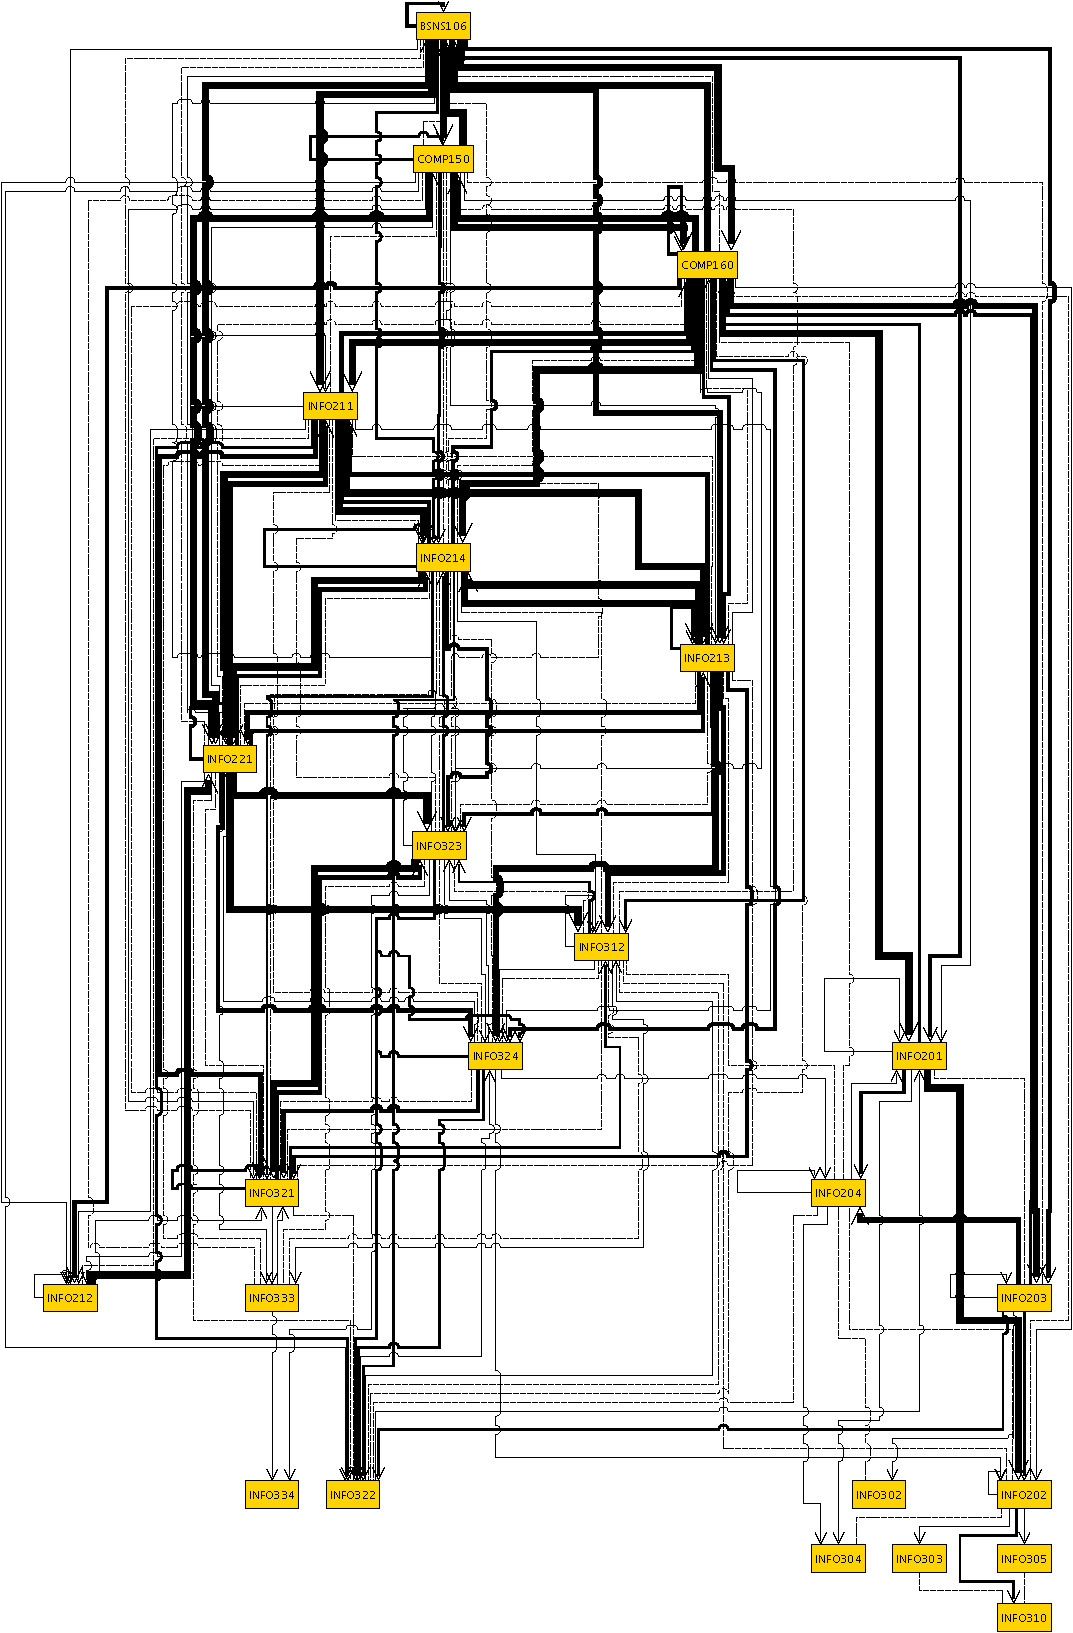
\includegraphics[height=6.5cm,keepaspectratio]{paper_sequence}
        \end{column}
    \end{columns}
\end{frame}


%%%%%%%%%%%%%%%%%%%%%%%%%%%%%%%%%%%%%%%%%%%%%%%%%%%%%%%%%%%%%%%%%%%%%%%%%%%%%%%%


\begin{frame}
    \frametitle{Data sources for student data}
    
    \begin{tikzpicture}[remember picture, overlay]
        \node[anchor=north east] (BO) at ($(current page.north east) - (1mm,2mm)$) {
            
\includegraphics[width=3.5cm,keepaspectratio]{BO.png}
        };
        \node[anchor=east] (eVision) at ($(current page.east) + (-1mm,7mm)$) {
            
\includegraphics[width=3cm,keepaspectratio]{eVision.png}
        };
        \node[anchor=south east] (ttrpt02) at ($(current page.south east) + (-1mm,3mm)$) {
            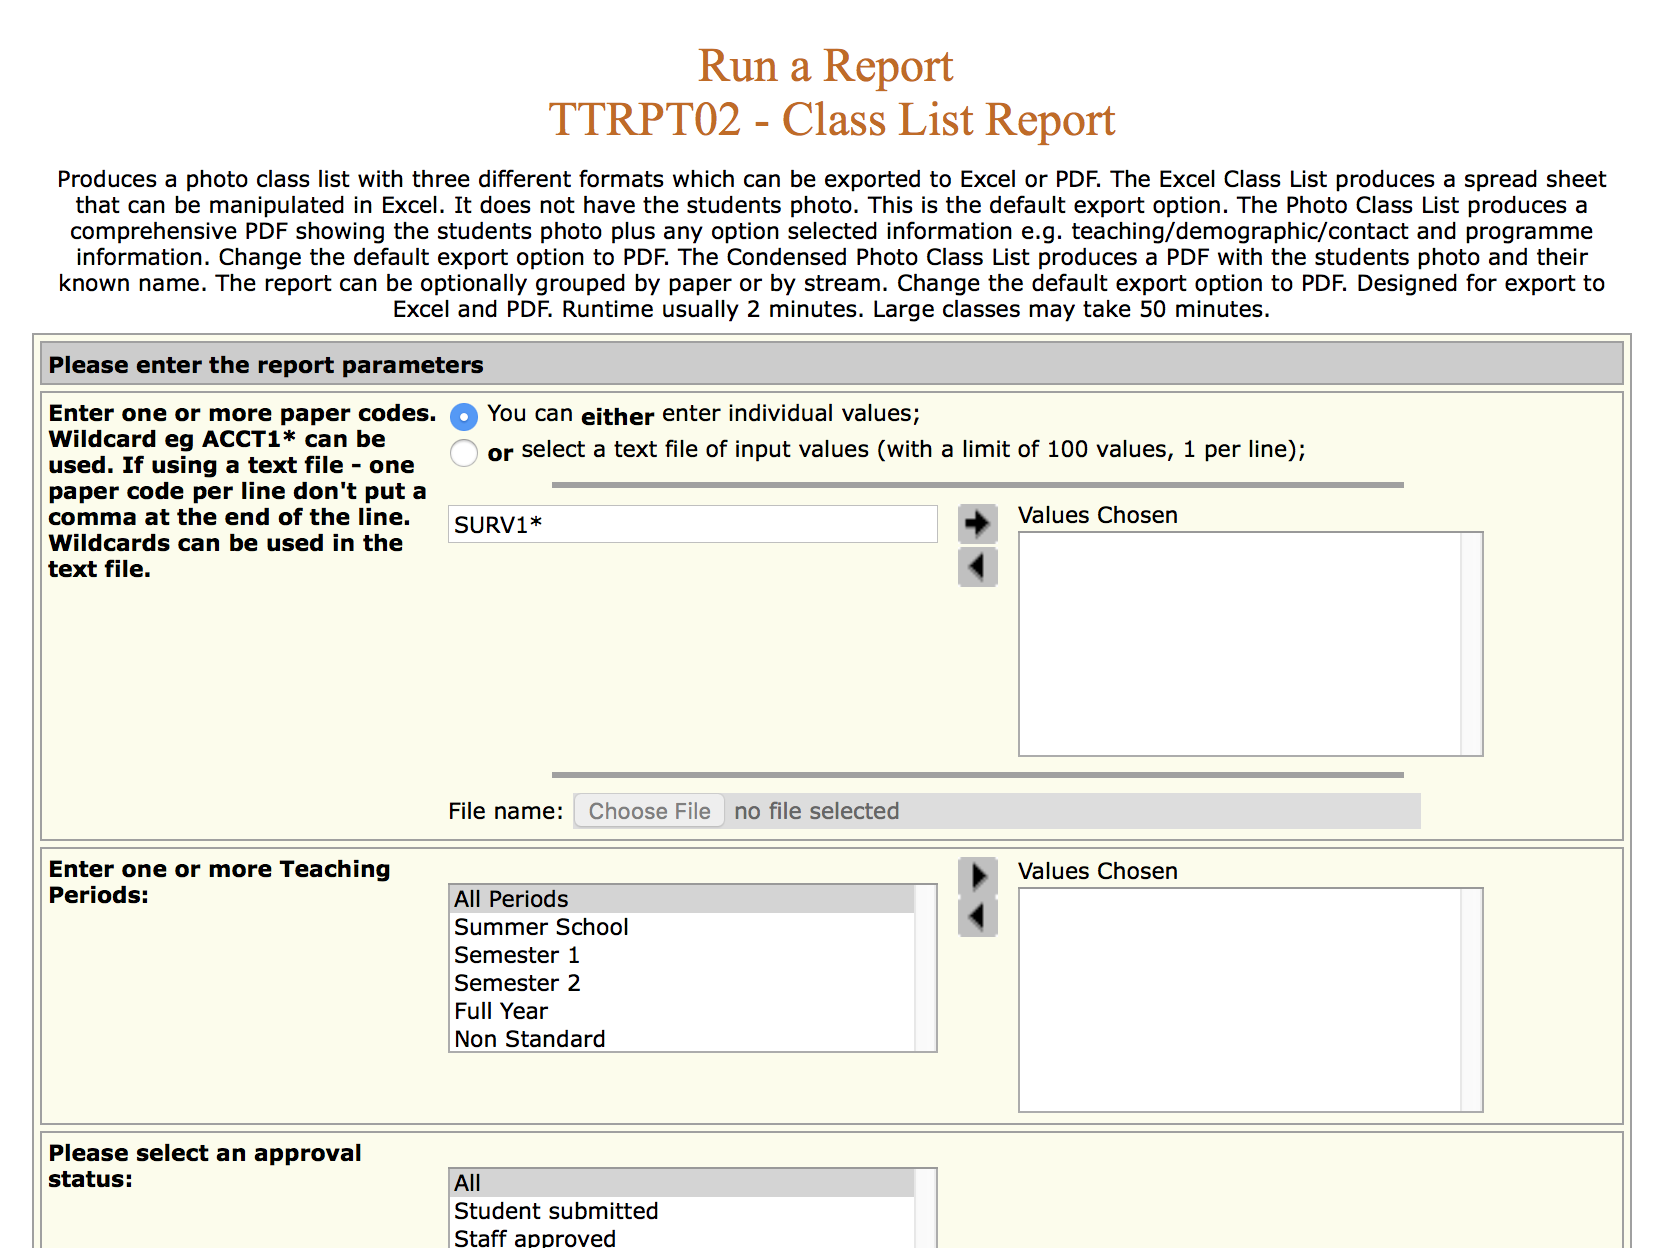
\includegraphics[height=2.8cm,keepaspectratio]{TTRPT02.png}
        };
    \end{tikzpicture}
    
    \begin{itemize}
        \item Mostly eVision via Business Objects. {\tiny (maybe Blackboard for internal assessment)}
        \begin{itemize}
            \item human readable (PDF \alert{\faFilePdfO}, Word \textcolor{structure}{\faFileWordO})
            \item “machine-readable” (CSV \faFileTextO, XLS \textcolor{green!50!black}{\faFileExcelO})
        \end{itemize}
    \end{itemize}
    \medskip
    
    \begin{tabular}{lp{8cm}}
        \structurebf{CARPT004}  &   paper, student, and enrolment data  \\
        \structurebf{TTRPT02}   &   enrolment and streaming data  \\
        \structurebf{EXRPT11}   &   final results and internal assessment {\tiny (Results I vs.\ II)}  \\
        \structurebf{SDRPT12}   &   student retention, including degree completion and annual workload  \\
        \structurebf{SDGPA01}   &   GPA data (per year, level,  \\
                                &   and overall)  \\
    \end{tabular}
\end{frame}


%%%%%%%%%%%%%%%%%%%%%%%%%%%%%%%%%%%%%%%%%%%%%%%%%%%%%%%%%%%%%%%%%%%%%%%%%%%%%%%%


\begin{frame}
    \frametitle{Typical problems encountered}
    
    \begin{itemize}
        \item Old formats (.xls) \(\Rightarrow\) long term preservation issues.
        
        \item Business Objects reports were developed ad hoc:
        \begin{itemize}
            \item overlapping content
            \item inconsistent parameter configuration
            \item output more likely to be designed for human readability
            \item can change without warning {\tiny (esp.\ after eVision rollout)}
        \end{itemize}
        
        \item No API access \(\Rightarrow\) no ad hoc querying.
        
        \item Reading delimited text is often easier. \faMehO
    \end{itemize}
\end{frame}


%%%%%%%%%%%%%%%%%%%%%%%%%%%%%%%%%%%%%%%%%%%%%%%%%%%%%%%%%%%%%%%%%%%%%%%%%%%%%%%%


\begin{frame}
    \frametitle{EXRPT11 “Tabular” report}
    
    \bigskip
    Stated as “must run in Excel” \(\Rightarrow\) intended to be \alert{machine readable}.
    \bigskip
    
    \centering
    \begin{tikzpicture}
        \node[anchor=south west] (ss) {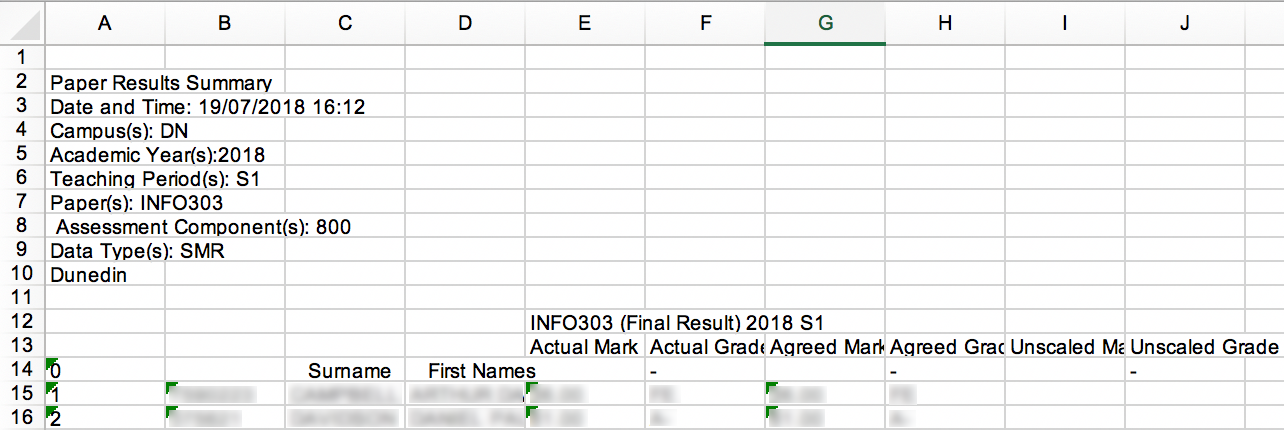
\includegraphics[width=0.95\columnwidth,keepaspectratio]{EXRPT11_Tabular}};
        \begin{uncoverenv}<2>
            \node[draw, ultra thick, ellipse, OU red, minimum width=1cm] (id) at (1.9cm,0.6cm) {};
            \node[draw, ultra thick, ellipse, OU red, minimum width=3cm, minimum height=0.7cm] (grades) at (5.8cm,0.7cm) {};
            \node[OU red] (wtf) at (3.5cm,-0.8cm) {\textbf{?!?!}};
            \draw[OU red, thick, -{Stealth}] (wtf) -- (id);
            \draw[OU red, thick, -{Stealth}] (wtf) -- (grades);
        \end{uncoverenv}
    \end{tikzpicture}
\end{frame}


%%%%%%%%%%%%%%%%%%%%%%%%%%%%%%%%%%%%%%%%%%%%%%%%%%%%%%%%%%%%%%%%%%%%%%%%%%%%%%%%


\begin{frame}
    \frametitle{EXRPT11 “Summary” report}
    
    \bigskip
    Stated as “must run in PDF” \(\Rightarrow\) \alert{not} intended to be machine readable.
    \bigskip
    
    \centering
    \begin{tikzpicture}
        \node (ss) {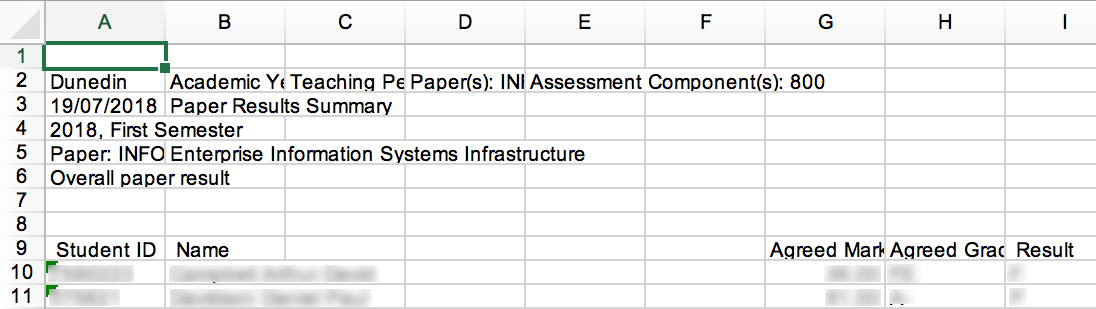
\includegraphics[width=0.95\columnwidth,keepaspectratio]{EXRPT11_Summary}};
        \node[OU red, below=5mm of ss] (huh) {\huge\textbf{!!!}};
    \end{tikzpicture}
\end{frame}


%%%%%%%%%%%%%%%%%%%%%%%%%%%%%%%%%%%%%%%%%%%%%%%%%%%%%%%%%%%%%%%%%%%%%%%%%%%%%%%%


\begin{frame}
    \frametitle{SDRPT12 mysteriously fixed itself}
    
    \bigskip
    \structurebf{\alt<2>{July 2018}{Early 2018}}
    \bigskip
    
    \centering
    \begin{tikzpicture}
        \node (broken) {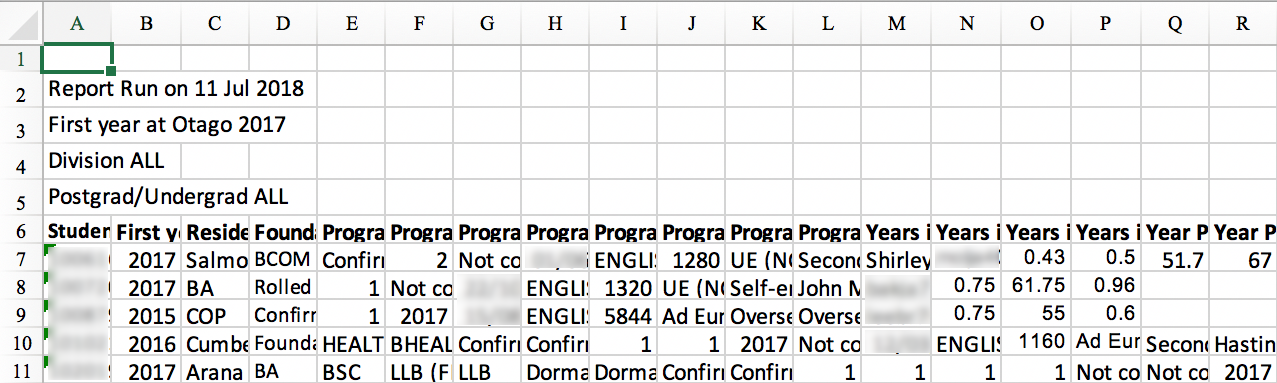
\includegraphics[width=0.95\columnwidth,keepaspectratio]{SDRPT12_bustificated}};
        \uncover<2>{\node (fixed) {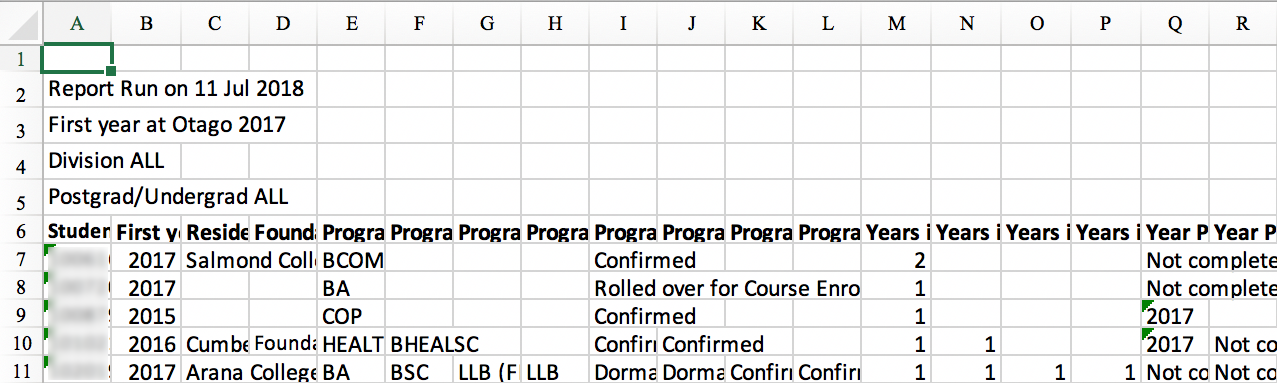
\includegraphics[width=0.95\columnwidth,keepaspectratio]{SDRPT12_fixed}};}
    \end{tikzpicture}
    \bigskip
    
    \footnotesize
    \uncover<2>{(This is good, as the only other source of completion data is the student transcript.)}
\end{frame}


%%%%%%%%%%%%%%%%%%%%%%%%%%%%%%%%%%%%%%%%%%%%%%%%%%%%%%%%%%%%%%%%%%%%%%%%%%%%%%%%


\begin{frame}
    \frametitle{So why are things still such a mess?}
    \framesubtitle{(WARNING: rampant speculation!)}
    
    \structurebf{Lack of demand/knowledge?}
    \begin{itemize}
        \item Technically naive data consumers don’t know it can be better?\tinyskip
        {\tiny (“you get that with computers”)}
        \item e.g., 3 pages of instructions to generate class email list vs.\ VBA app that queries student AD/LDAP.
        \item How can we better inform/educate non-technical end users?\tinyskip
        {\tiny (or will the problem eventually solve itself?)}
    \end{itemize}
    \bigskip
    
    \structurebf{Apathy/cynicism?}
    \begin{itemize}
        \item Those in the know already have “good enough” workarounds?
        \item “ITS will never do anything about this.”
        \item Do we need more concerted collective action?\tinyskip
        {\tiny (see lack of demand above)}
    \end{itemize}
\end{frame}


%%%%%%%%%%%%%%%%%%%%%%%%%%%%%%%%%%%%%%%%%%%%%%%%%%%%%%%%%%%%%%%%%%%%%%%%%%%%%%%%


\begin{frame}
    \frametitle{So why are things still such a mess?}
    \framesubtitle{(WARNING: rampant speculation!)}
    
    \structurebf{Ancient software/interfaces?}
    \begin{itemize}
        \item e.g., Business Objects.
        \item Can we convince the powers that be to provide something more modern? {\tiny (e.g., REST API, service bus, …)}
    \end{itemize}
    \bigskip
    
    \structurebf{ICT support indifferent/inflexible/unaware to needs?}
    \begin{itemize}
        \item “We’ll do it if you pay for it.” {\tiny (e.g., custom Business Objects reports)}
        \item “Why would you need (to do) that?”
        \item “There shouldn’t be so many feral systems.”
        \item “Opening up our systems like that is too risky.”
        \item Focused on bigger projects/needs?
    \end{itemize}
\end{frame}


%%%%%%%%%%%%%%%%%%%%%%%%%%%%%%%%%%%%%%%%%%%%%%%%%%%%%%%%%%%%%%%%%%%%%%%%%%%%%%%%


\begin{frame}
    \centering\bigskip\bigskip\bigskip
    \Huge\structurebf{Thank you!}
    \bigskip\bigskip
    
    \Large\structurebf{Floor open for questions, discussion, rants \faSmileO}
\end{frame}


%%%%%%%%%%%%%%%%%%%%%%%%%%%%%%%%%%%%%%%%%%%%%%%%%%%%%%%%%%%%%%%%%%%%%%%%%%%%%%%%


\end{document}
